\documentclass{article}
\usepackage[a4paper, margin=1in]{geometry}

\usepackage[french]{babel}
\usepackage{listings}
\usepackage[utf8]{inputenc}
\usepackage[hidelinks]{hyperref}
\usepackage{graphicx}
\usepackage{shorttoc}
\usepackage{listings}
\usepackage{caption}
\usepackage{amssymb}
\usepackage{verbatim}
\lstset{language=java}

\newcommand{\source}[1]{\caption*{Source: {#1}} }

\title{Projet Cloud - DaarSearch}
\author{Julien Bissey, Mohammed-Achraf Charif}

\begin{document}

\maketitle

\section*{Introduction}
\addcontentsline{toc}{section}{Introduction}

Ce document est notre rapport de projet Cloud pour l'UE DAAR. Nous l'avons codé avec le language Java. Dans ce projet, nous cherchons d'abord à implémenter un moteur de recherche sur une base de documents textuels, pour ensuite le rendre accessible sur le web sous la forme d'une application.\\
Lorque que l'utilisateur donne un mot, ce moteur de recherche doit pouvoir rendre la liste des livres contenant ce mot, ainsi qu'une liste de suggestions de livres proches des meilleurs résultats.\\
Les sources de notre projet sont disponibles ici : \url{https://github.com/Ishyro/DaarSearch}.\\
Pour classer les résultats et déterminer quels livres suggerer, nous avons choisi de placer les livres de notre bibliothèque dans un graphe géométrique, dont les arrêtes correspondent à la distance de Jaccard entre les différents livres. Ce critère nous permet de décider quels livres nous pouvons suggérer, il nous suffira de regarder quels sont les livres les plus proche de celui qui nous concerne. A l'aide de ce graphe, nous pouvons également définir un critère de centralité afin de classer les livres en fonction de leur importance dans le graphe. Ce classement nous permet de déterminer l'ordre dans lequel nous trierons la liste de résultats obtenue par l'utilisateur.

\section{Recherche de mot}

Une des contraintes de notre projet est de pouvoir rechercher des expressions régulières (notées RegEx) en plus des mots simples. Cependant, une recherche de RegEx est moins performante qu'une simple recherche de mot et prend donc davantage de temps à se réaliser. C'est pourquoi nous utilisons deux algorithmes différents pour faire ces deux types de recherches, même s'il est tout à fait possible de rechercher un simple mot avec notre algorithme de recherche de RegEx.

\subsection{Knuth-Morris-Pratt}

Pour rechercher les simples mots, nous utilisons l'algorithme Knuth-Morris-Pratt, qui est très performant car il peut trouver un mot en une seul lecture du texte ($0(n)$), là où un algorithme naif devrait faire des rollbacks à chaque fois qu'il ne matcherait pas la lettre attendue.\\

On peut décomposer cet algorithme en deux étapes. La première étape consiste à parcourir le texte et à associer à ce texte un tableau d’entier indiquant des indices de décalages, qui fournissent une information sur la position a laquelle placé le curseur de parsing en cas de non matching de le RegEx
recherchée. Ces indices sont calculés en fonction du motif, et des caractères précédemment parcourus.\\

Après cette étape, on effectue l’algorithme egrep like a proprement parlé et chaque fois que la correspondance échoue, on regarde l’indice correspondant et on reprend à l’emplacement correspondant. Par exemple si l’on cherche le motif sargon et qu’on effectue une vérification sur sarah, les 3 premiers caractères vont correspondre mais une fois arrivé au deuxième a de sarah, le test de correspondance échoue. On va regarder l’indice correspondant et sachant que lors de la première étape nous avonsconstaté qu’il n’y avait pas d’autre prefixe potentiel dans sarah, on transmet l’information en indiquant qu’on peut recommencer la vérification à partir du h ce qui évite un rollback au niveau du premier a.

\newpage

\subsection{Automate d'Aho-Ulman}

Pour la recherche de RegEx, nous avons utilisé l'algorithme sans doute le plus utilisé pour résoudre ce type de problème : les automates décrits dans livre d’Aho-Ullman chapitre 10 \cite{AhoUllman}. Cette solution répond à la problématique suivante : comment rechercher un motif dans un texte de manière déterministe.\\
Pour se faire nous souhaitons prendre en entrée une expression régulière définissant le motif recherché et un texte dans lequel la recherche doit être effectuée.\\

\begin{itemize}
\item IN : String RegEx, String Text
\item OUT : String Lines in the Text matching with the RegEx\\
\end{itemize}

Cette méthode se décompose en quatre étapes. La première consiste à prendre l’expression régulière en entrée et à la traduire en arbre de RegEx plus facile à parcourir pour notre programme. Pour se faire il faut traiter chaque composant de notre grammaire séparément. Nous parcourons donc la RegEx et pour chaque caractère
rencontré on réagence l’arbre RegEx pour respecter la traduction. Voici un exemple concret illustrant ces propos :

\begin{figure}[!h]
  \centering
  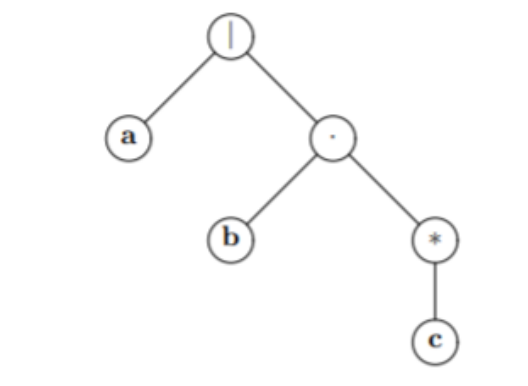
\includegraphics[width=.3\paperwidth]{abc*.png}
  \caption{Arbre correspondant à l’expression a | bc*}
\end{figure}

\begin{figure}[!h]
  \centering
  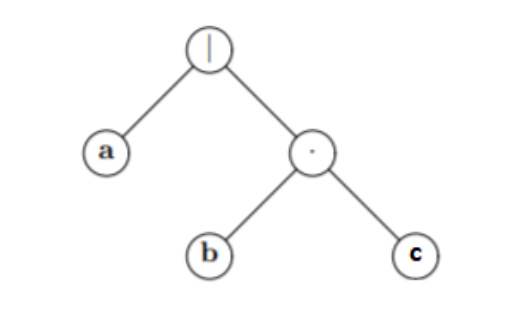
\includegraphics[width=.3\paperwidth]{abc.png}
  \caption{Arbre correspondant à l’expression a | bc}
\end{figure}

Cette étape implique donc la manipulation d’arbre et certains rollbacks pour modifier les liens de parentés des nœuds, car le parsing n’est pas prédictif, on ne peut donc pas anticiper sur le prochain caractère. Dans le pire des cas on a une complexité en $O(2^m)$ pour la construction de l’arbre, m étant la taille de la RegEx. La deuxième étape consiste a transformé ce RegEx Tree en automate, qui est dans notre cas non pas une matrice indiquant tous les états et toutes les transitions entre ces états, mais un modèle plus orienté objet avec une liste de transitions. Pour cela on commence par utiliser les epsilons transitions pour expliciter la totalité du comportement de notre automate puis on supprime ces epsilons transitions pour obtenir une minimisation de notre automate en utilisant la règle fermeture. Une fois cette étape réalisée, on peut appliquer la recherche de motif sur l’automate minimal en parcourant les états d’une transition a une autre, en concluant dans le cas ou l’on parvient à atteindre un état final depuis un état initiale.\\

Au final, cette méthode permet de trouver des mots en $O(n^2)$ ce qui est problématique pour des textes assez longs mais aussi pour de grosses RegEx étant donné la présence de rollbacks. C'est donc pour cela que l'utilisation de l'algorithme KMP est préférable pour un simple mot.

\section{Bibliothèque et graphe}

Afin de tester et déployer ce projet, nous avons utilisé des livres réels écrits en anglais. Nous nous sommes proccuré $1000$ livres, rendus disponibles par le projet Guttemberg \cite{Guttemberg}. Ainsi, à chaque recherche, nous allons devoir parcourir les $1000$ livres. il est donc judicieux de chercher à faire des optimisations sur les fichiers que nous allons lire.\\

De plus, afin de calculer nos critères pour ordonner les livres, et suggérer des livres à l'utilisateur, nous allons utilisé un structure d'arbre où chaque noeud sera un livre, relié aux autres par sa distance de Jaccard avec eux.

\subsection{Indexage}

Puisque ce moteur de recherche doit uniquement rendre le nom des livres où le mot est détecté, et non pas les phrases où ce mot est detecté, il n'est pas nécessaire de faire les recherches dans le texte original. Nous avons donc utiliser des fichiers d'index, qui contiennent chaque mot d'un livre et son nombre d'occurence. Un tel fichier peut avoir une taille $O(log(n))$ comparée à la taille n du texte original, même si ce cas n'arrivera jamais pour un texte écrit en anglais usuel, pusqu'il nécessite que chaque mot ait le même nombre d'occurences dans le texte. On remarque tout de même une nette amélioration du temps de calcul pour effectuer une recherche sur ces indexes.\\

Afin de créer ces indexes, nous avons d'abord transformé les textes en arbres radix afin de compter les occurences de tous les mots de manière efficace en une seule lecture du texte, même si la construction de l'arbre est coûteuse. Nous avons ensuite simplement trié les mots en fonction de leur nombre d'occurences. Nous ignorons les $100$ mots les plus fréquents de la langue anglaise, car on supposent qu'ils se sont pas intéressants pour l'utilisateur (savoir que tous les 1000 livres contiennent le mot \textit{the} ne devrait pas beaucoup l'avancer).

Un radix tree peut se définir comme un arbre préfix compressé. En effet, cet arbre suit le même principe, mais une arrête peut contenir une suite de caractères dans le cas où tous les mots suivants ce chemin de l'arbre ont cette suite de lettres en commun. Cela permet de réduire le coût de l'arbre en mémoire d'une part, mais également de réduire le coût en temps de calcul des opérations de recherche dans l'arbre.

\begin{figure}[!h]
  \centering
  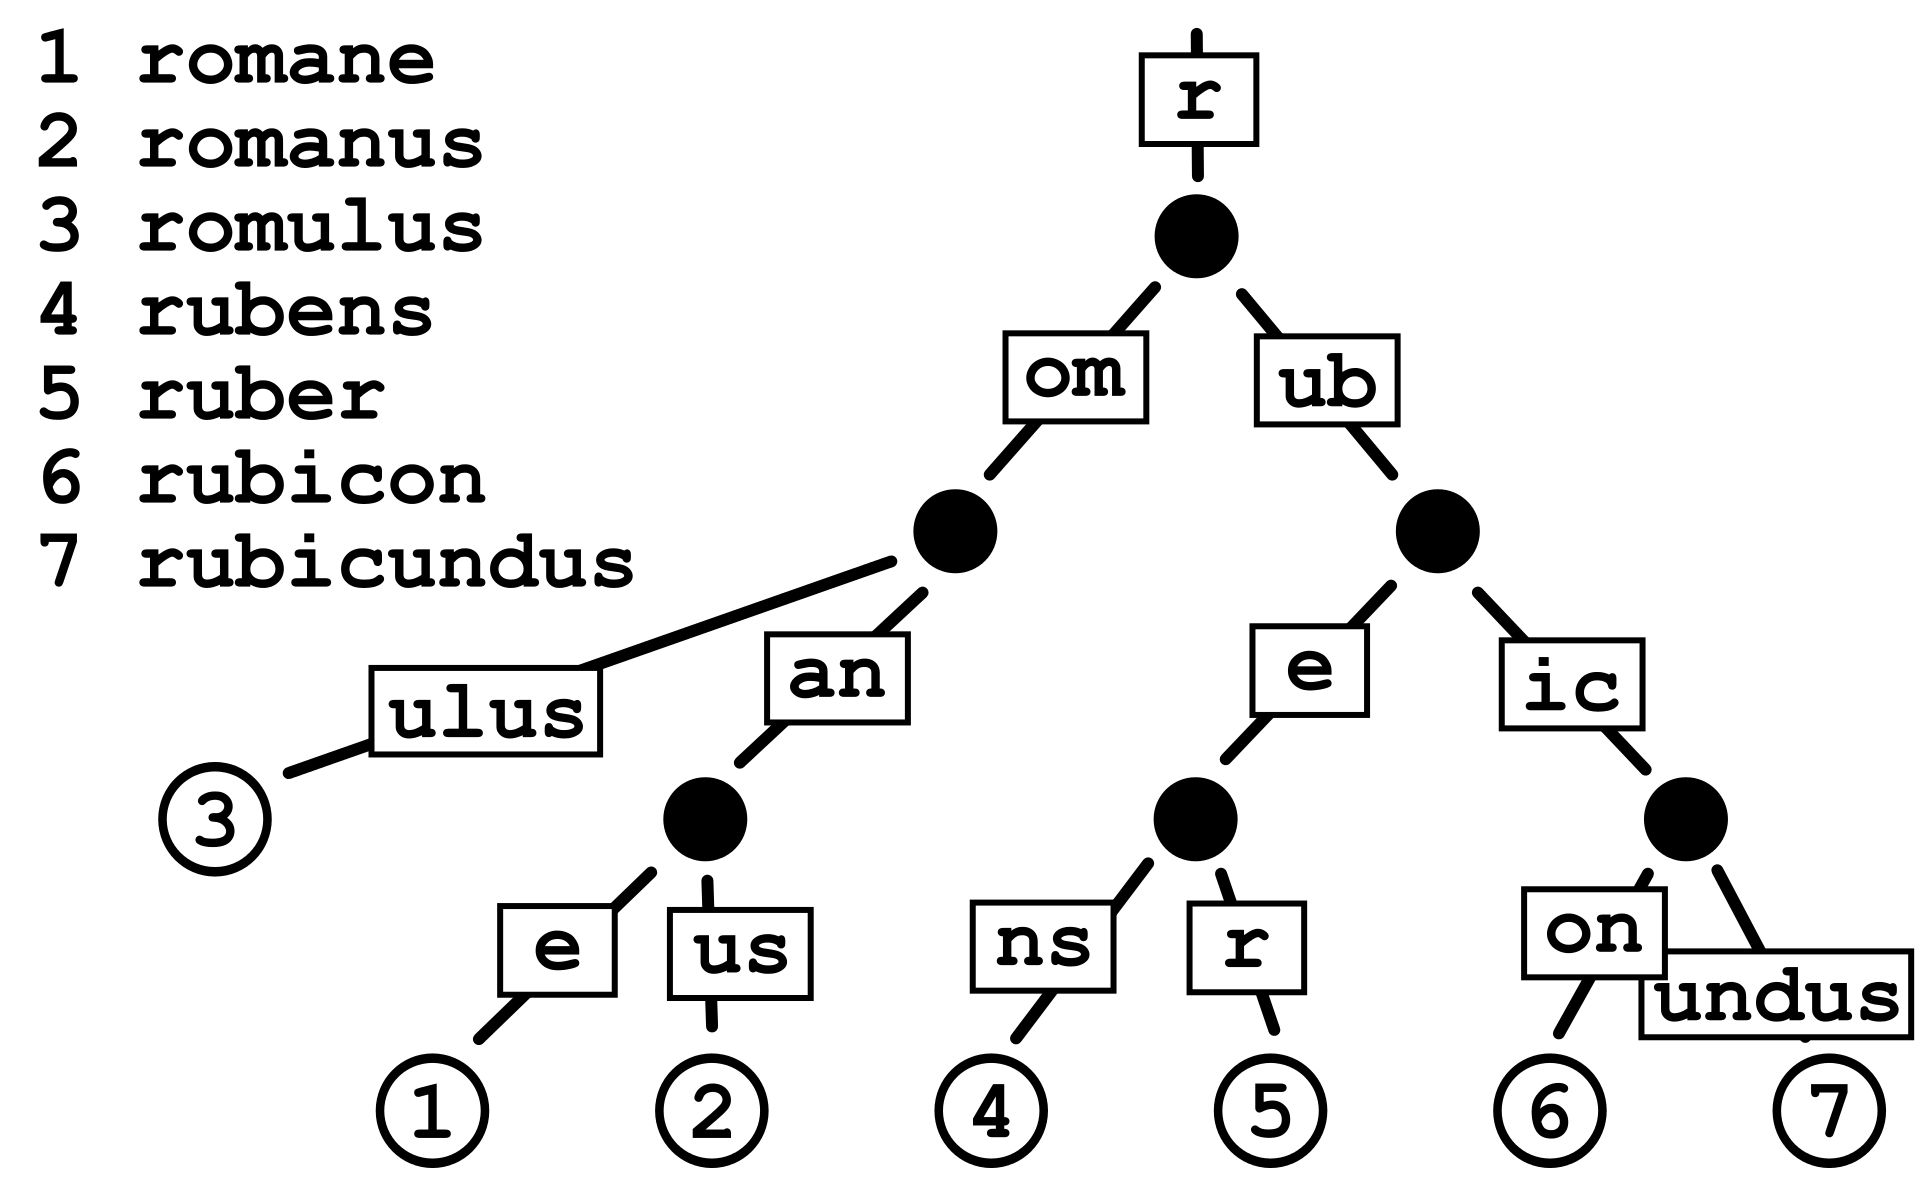
\includegraphics[width=.3\paperwidth]{radix_tree.png}
  \caption{Exemple d'arbre radix}
\end{figure}

\subsection{Distance de Jaccard}

\textit{Note : suite à une erreur, les distances de Jaccard ainsi que la betweenness ont été calculées à partir de mauvais fichiers d'index. L'aspect théorique autour de ces calculs dont nous allons discuter ici reste pertinent, mais les résultats expérimentaux que nous pouvons en tirer le seront moins. De plus, même si les fichiers d'index ont été corrigés, ils n'ont pas pu être déployés sur le serveur, faute de temps. Les recherches ne fonctionneront donc pas sur tous les mots.}\\

A partir de ces fichiers d'index, nous pouvons également calculer la distance de Jaccard entre deux livres. C'est un critère visant à déterminer la proximité entre deux textes se basant sur les différences de vocabulaire entre les deux textes. Elle se calcule à partir de cette formule:
$J(A,B) = \frac{|A \cup B| - |A \cap B|}{|A \cup B|}$. On a en effet uniquement besoin de savoir quels mots sont contenus dans chaque livre. Dans les faits, on va repasser par des arbres radix, car ils nous ferons gagner du temps sur les recherches, mais on peut les construire plus rapidement à partir des indexes qu'à partir des textes originaux.\\

Une fois qu'on a obtenu la distance de Jaccard entre chaque texte, on va pouvoir créer notre graphe. On considère que deux livres sont liés uniquement si leur distance de Jaccard est inférieure à $0.7$ (valeur arbitraire qui semble bien fonctionner). En effet, avec cette valeur, le graphe contient $78876$ arrêtes, $58$ livres sur $1000$ se retrouvent isolés dans le graphe, mais certains livres ont déjà plus de $300$ voisins, il est donc préférable de ne pas rendre ce seuil plus large.

\subsection{Betweenness}

Une fois ce graphe obtenu, on peut s'attaquer au calcul d'un critère de centralité afin de trier nos livres par ordre d'importance. Nous avons choisi la betweenness.
Pour chaque noeud v, on calcule $g(v)= \sum_{s \neq v \neq t}\frac{\sigma_{st}(v)}{\sigma_{st}}$ avec  $\sigma_{st}$ le nombre total de chemins les plus courts entre $s$ et $t$, et  $\sigma_{st}(v)$ le nombre de ces chemins passant par $v$.\\

Pour calculer la betweenness, on va donc d'abord devoir calculer l'ensemble des plus courts chemins de notre graphe. L'algorithme qui nous semble le plus judicieux pour ce cacul est celui de Floyd-Warshall, légèrement modifié, car on veut détecter tous les plus courts chemins, et non pas un seul par paire de noeuds. De plus, on va introduire un seuil pour considérer deux valeurs très proches comme égales, puisque les poids des arrêtes sont des flottants (distance de Jaccard). On va arbitrairement choisir $0.0025$.\\

Nous allons nous intéresser à quelques unes des valeurs obtenues (Même si elles sont basées sur de mauvais index, le passage de la distance de Jaccard à la betweenness garde tout son sens, et on peut tout de même en tirer des conclusions).\\

\begin{itemize}
\item Livre 10728 : Ce livre possède la betweenness maximale ($60133,971429$), car il possède également un grand nombre de voisins ($373$). Il s'agit du livre  \textit{Christie, the King's Servant} de Mrs. O.F. Walton. Si l'importance de ce livre peut sembler suprenante... cela est dû à notre erreur sur les index.
\item Livre 10794 : Ce livre possède le plus grand nombre de voisins ($469$), et la troisième plus grande betweenness ($29681,702381$).
\item Livre 10454 : même nombre de voisins, mais betweenness plus basse, uniquement la vingt-et-unième ($13723,730952$).
\item Livre 10841 : l'un des nombreux livres avec une betweenness à $0$, il a tout de même $5$ voisins.\\
\end{itemize}

On voit donc que la betweenness est un critère visant à déterminer l'importance réelle du noeud au sein du graphe entier, et pas simplement à son importance dans un sous graphe limité comme le ferait un simple tri en fonction du degré des noeuds. Un tel tri donnerait évidemment un résultat similaire, car le lien entre les deux valeurs est trivial, mais la précision supplémentaire apportée par la betweenness est non négligeable.

\newpage

\section{Choix des technologies web}

Pour déployer notre projet, nous avons choisi Angular, Node.js et Jetty Jersey.\\

\begin{itemize}
\item Angular : un framework complet bien documenté qui répond à toutes nos attentes.
\item Node.js : facile à utiliser, et offre de bonnes performances.
\item Jetty Jersey : facile à utiliser, léger et rapide.\\
\end{itemize}

\section*{Conclusion}
\addcontentsline{toc}{section}{Conclusion}

Nous avons pu créer un moteur de recherche sur une base de documents textuels fonctionnelle, capable de trier les résultats par ordre d'importance, et de suggérer d'autres lives à l'utilisateur en fonctions de ces résultats. Nos critères utilisés, la distance de Jaccard et la betweenness, peuvent ne pas sembler optimaux pour ordonner des textes littéraires, car ils ne prennent pas en compte des aspects comme le succès d'un livre, l'appartenance à une série de plusieurs tomes... Mais ils ont cependant un grand avantage : ils sont objectifs.\\
Cependant, on pourrait envisager une amélioration pour la distance de Jaccard. En effet, elle exprime la différence de vocabulaire, mais elle ne fait pas intervenir les données numériques de ce vocabulaire. Elle accorde la même importance à un mot trouvé une fois qu'à un mot trouvé mille fois dans un texte.\\

On pourrait envisager d'utilser la distance de Levenshtein, qui s'intéresse au nombre d'insertions, suppresions et remplacements de caractères nécessaires pour rendre deux textes égaux, mais on aurait encore deux problèmes :\\

\begin{itemize}
\item Il n'y a aucune raison d'accorder de l'importance à l'ordre des textes.
\item De même, la taille du texte n'est pas importante, c'est plutôt la densité des mots dans le texte qui nous intéresse.\\
\end{itemize}

Trouver un critère pour determiner la proximité entre deux textes est en réalité un problème extrêmement complexe, c'est pourquoi même si la distance de Jaccard n'est pas optimale, elle reste satisfaisante pour nos besoins.


\bibliography{biblio}{}
\bibliographystyle{unsrt}
\addcontentsline{toc}{section}{Bibliographie}

\newpage

\tableofcontents
\addcontentsline{toc}{section}{Table des matières}

\end{document}
